%*********************第一章******************
\chapter{绪论}
基于加速器的异构系统是指采用不同功能或性能的计算设备,通过一定互联而构成的计算机系统,其中一种计算设备的计算能力强于传统的通用处理器,被称为加速器,用于实现对应用程序需要密集计算部分的计算加速。典型的加速器包括数字信号处理器(DSP)、面向通用计算的图像处理器(GPU)、众核协处理器(MIC)以及硬件加速器(FPGA)等。

基于拥有大量计算核的 GPU 和 MIC 进行加速的异构计算的出现和迅猛发展有力地推动了高性能计算领域和科学研究。基于加速器搭建异构超级计算机已经成为高性能计算领域一个重要的发展趋势,天河1A和天河2号分别是基于GPU和MIC加速器的超级计算机,它们都曾经位列世界超级计算机TOP500之首。各种异构平台的出现为高性能计算以及各类应用提供了很好的机遇,同时,针对异构系统的并行优化成为挑战。

本课题选取了科学计算领域和人工智能领域的相关应用,一个是心脏组织的3D模拟,另一个是卷积神经网络计算,根据它们各自的计算特点,将它们分别映射到基于MIC的异构平台和基于GPU的异构平台中,在映射过程中解决了一系列并行优化问题。
\section{研究背景}
异构平台应用越来越广泛,服务器和集群系统都偏向采用异构体系结构,各种异构硬件平台可以相应解决不同的应用领域。科学计算领域对计算需求比较大,需要大规模集群系统才能满足计算的需求。而对于近两年比较火的人工智能领域,也属于计算密集型应用,在异构平台的服务器上可以得到满足。本课题选取了心脏组织模拟以及卷积神经网络应用作为科学计算和人工智能领域的研究例子,对异构平台并行优化技术进行研究。本节首先介绍异构平台及异构编程,然后介绍了心脏组织模拟以及卷积神经网络对计算的需求,最后介绍了应用在异构并行计算中可能面临的挑战。

\subsection{异构平台及异构编程}
       \subsubsection{加速器发展趋势}
       近年来,集成电路和体系结构的发展,使得处理器性能呈指数增长。摩尔定律指出,集成电路的集成度每18个月翻一倍,而单芯片中晶体管数接近十亿个,频率达到GHz。VLSI工艺的发展给处理器体系结构的发展提供动力。传统的处理器研究主要目标是提高单芯片的性能,因此,主要采用指令级并行(ILP)技术和提高处理器工作频率等方法提高单处理器的性能。这两个技术带来的问题就是功耗和散热的问题,这些问题又导致芯片的可靠性下降。这些因素使得摩尔定律遇到瓶颈。
       
       研究人员开始转向多核/众核处理器的研究,多核或者众核技术的研究打破了摩尔定律受限的瓶颈。多核/众核处理器设计的思想是在单个芯片中集成多个简单的处理器核并行工作,多核/众核处理器的设计不仅延续了指令级并行的特点还支持开发数据级和任务级的并行,多核/众核处理器工作的频率可以低于传统的单核频率,消除了因频率过高带来的可靠性以及能耗的问题。由于多核/众核处理器中小核设计比传统的单核处理器设计来得简单,这降低了处理器设计的难度,提高了设计效率。
       
       多核革命引来了微处理器厂商对多核/众核处理器的研究。2005年多家处理器厂商推出了双核CPU,并陆续推出四核、八核等多核CPU。而在高性能计算领域,英伟达公司推出了面向通用计算的GPU众核处理器,GPU中集成了数百个计算核心,采用CUDA编程框架,程序员逻辑上可以设置成千上万个线程,这些线程执行相同的硬件指令,只是处理不同的输入数据。GPU大量密集的计算资源使其具有强大的计算能力,目前,英伟达比较新的GPU峰值性能高达10Tflops,远超当前的多核CPU的性能。2012年,Intel公司推出了MIC架构的众核协处理器Xeon Phi,该处理器大概有60多个计算小核,同时支持大概200多个硬件线程执行,双精度浮点性能超过1Tflops。与通用处理器相比,众核处理器在性能功耗比上具有明显的优势。
       
       从巨型机到普通PC机,多核/众核处理器已经被广泛使用于各个领域。特别是高性能计算领域,世界上大部分巨型机系统都采用GPU和MIC等众核加速器作为协处理器,以较高的性能功耗比,推动了高性能计算的发展。

       \subsubsection{加速器体系结构}
       目前的加速器类型众多,典型的有DSP、GPU、FPGA以及Intel MIC。本课题研究基于的硬件平台主要是NVIDIA GPU以及Intel MIC异构平台。下面分别对这两种体系结构进行介绍。
       
       1. GPU体系结构
       
       2009年,随着NVIDIA公司推出了Fermi架构GPU,高性能计算从此进入异构计算时代,随后陆续推出Kepler架构、Maxwell架构以及Pascal架构的GPU。下面以最新的Pascal体系结构为例对GPU体系结构进行介绍,图\ref{fig:pascal1080}是Pascal架构GPU的结构示意图。Pascal GPU由不同配置的GPCs(Graphics Processing Clusters),SMs(Streaming Multiprocessors)以及存储控制器。SM详细结构如图\ref{fig:pascalsm}所示。对于Geforce GTX 1080 GPU来说,其包含4个GPCs,20个SMs以及8个存储控制器,每个GPCs中含有5个SMs,每个SM内部又含有128个CUDA核心,256KB的寄存器文件大小,96KB的共享存储,48KB大小的L1 cache。GTX 1080 GPU单精度浮点峰值性能可达8.9TFlops,支持多达32GB的DDR5存储空间,访存带宽高达320 GB/s 。此外GTX 1080 GPU支持Nvlink技术,可以支持CPU和GPU间以及GPU与GPU间高速的数据传输,该项技术对某些通信频繁的应用比如深度学习具有很好的效果。
       \begin{figure}[ht!]
	\centering
	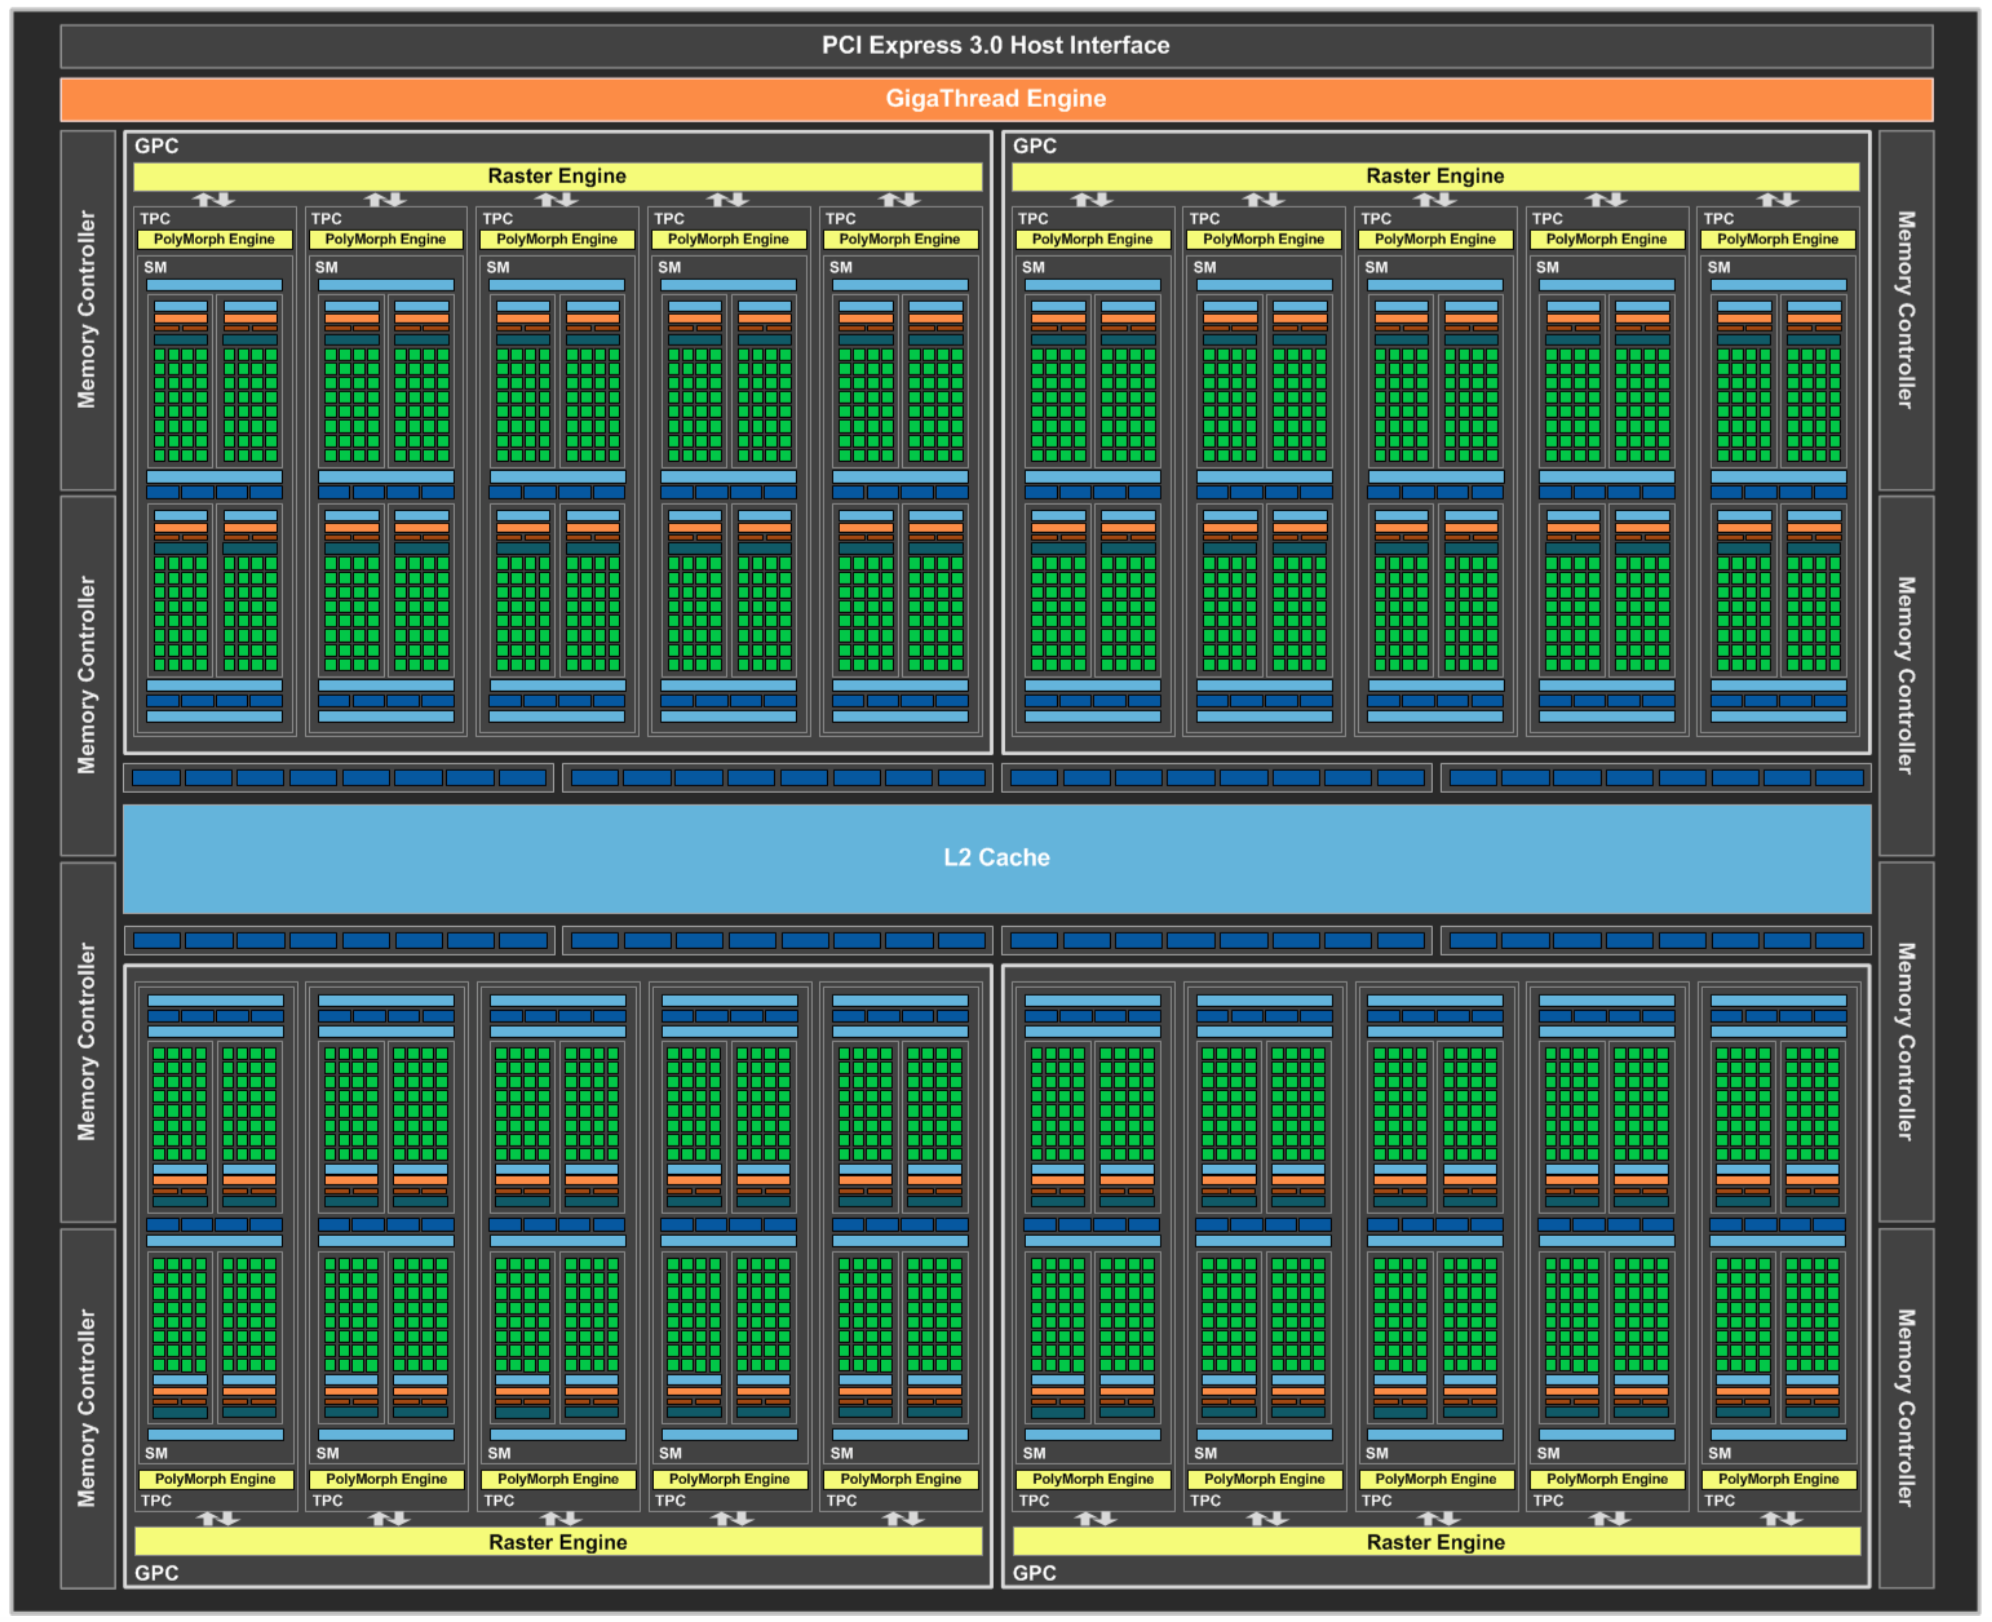
\includegraphics[width=0.9\linewidth]{figs/pascal_gp104_block_diagram.png}
	\caption{GTX 1080 GPU体系结构\upcite{gtx1080}}
	\label{fig:pascal1080}
	\end{figure}
	
	\begin{figure}[ht!]
	\centering
	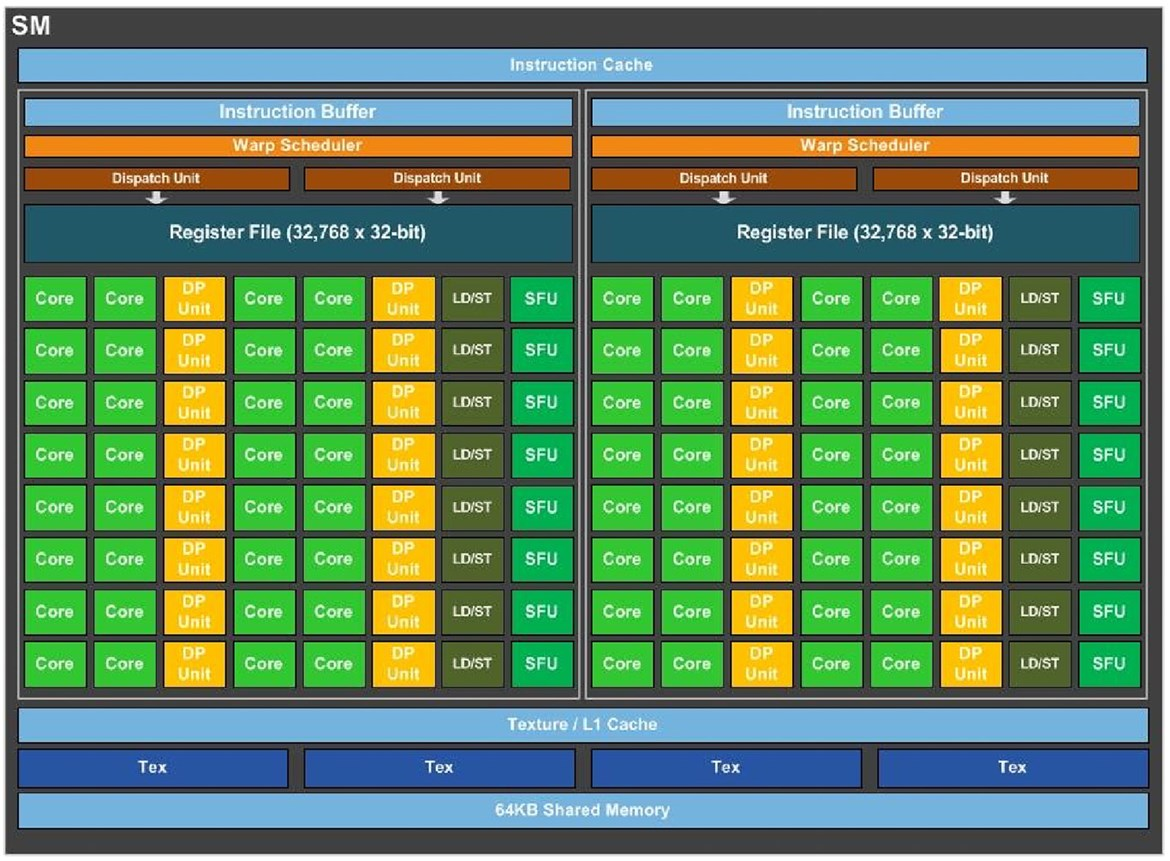
\includegraphics[width=0.9\linewidth]{figs/pascalgpu.jpeg}
	\caption{GTX 1080 GPU 中SM的体系结构\upcite{gtx1080}}
	\label{fig:pascalsm}
	\end{figure}
             
       表\ref{GPUProperty}是NVIDIA公司最近几年推出的各个体系结构的GPU的特点比较。从表中可以看出各种体系结构的GPU差别以及发展趋势,GPU芯片发展工艺越来越精细,因此集成的晶体管数量越来越多,而每个芯片内的CUDA核心数量从Fermi架构的512个提高到Pascal架构的3840个,峰值性能提升了近10倍,而功耗并没有提高多少,计算性能功耗比得到大大提高。GPU体系结构不仅计算能力不断提高,访存带宽也相应提高了很多。综合这些特点变化,GPU体系结构无论从计算能力还是功耗方面优势都在不断增强。
       
       \begin{table}[]
       \centering
       \caption{各代GPU体系结构特点比较}
       \label{GPUProperty}
       \begin{tabular}{|c|c|c|c|c|}
       \hline
       \textbf{GPU Architecture} & \textbf{NVIDIA Fermi}       & \textbf{NVIDIA Kepler}  & \textbf{NVIDIA Maxwell} & \textbf{NVIDIA Pascal} \\ \hline
       GPU Process & 40nm & 28nm  & 28nm & 16nm   \\ \hline
       Flagship Chip & GF110 & GK210  & GM200 & GP100   \\ \hline
       GPU Design & SM & SMX  & SMM & SMP   \\ \hline
       Maximum Transistors & 3.00 Billion & 7.08 Billion  & 8.00 Billion & 15.3 Billion   \\ \hline
       Maxium Die Size & 520${mm^2}$ & 561${mm^2}$  & 601${mm^2}$ & 610${mm^2}$   \\ \hline
       SM Per Compute Unit & 32 SPs & 192 SPs  & 128 SPs & 64 SPs   \\ \hline
       Maxium CUDA Cores & 512 CCs & 2880 CCs  & 3072 CCs & 3840 CCs   \\ \hline
       FP32 Compute & 1.33 TFLOPs & 5.10 TFLOPs  & 6.10 TFLOPs & 12 TFLOPs   \\ \hline
       FP64 Compute & 0.66 TFLOPs & 1.43 TFLOPs  & 0.2 TFLOPs & 6 TFLOPs   \\ \hline
       Maximun VRAM & 1.5 GB GDDR5 & 6 GB GDDR5  & 12 GB GDDR5 & 16/32 GB HBM2   \\ \hline
       Maxium Bandwidth & 192 GB/s & 336 GB/s  & 336 GB/s & 720 GB/s~1 TB/s   \\ \hline
       Maxium TDP & 244 W & 250 W  & 250 W & 300 W   \\ \hline
       
      \end{tabular}
      \end{table} 
       
       2. MIC体系结构
       
       与GPU处理器相当的众核处理器还有Intel公司推出的MIC众核处理器,第一代架构为Knights Ferry,第二代架构为Knights Corner,发布的产品名称为Intel Xeon Phi协处理器,天河2号超级计算系统采用的就是Intel Xeon Phi协处理器,并且每个节点装配了3个Phi协处理器,下面对通过Knights Corner架构来了解MIC加速器的体系结构。如图\ref{fig:knc_arch}所示:
           \begin{figure}[ht!]
	\centering
	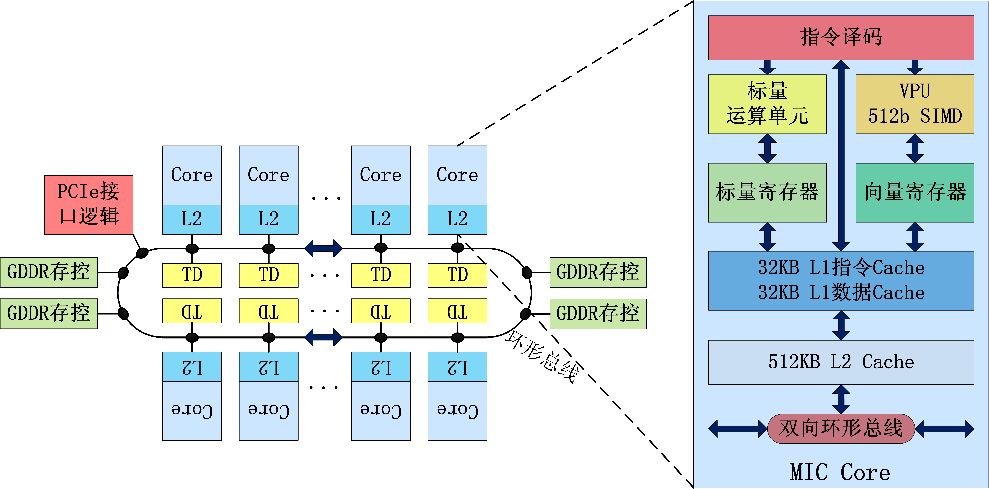
\includegraphics[width=0.9\linewidth]{figs/KNC_arch}
	\caption{Knigts Corner架构的MIC加速器体系结构图}
	\label{fig:knc_arch}
	\end{figure}

       MIC处理器中包含50+的微处理器核,众多的微处理器小核通过集成在单个芯片中,通过环形的总线互联。MIC处理器中的每个小核都是功能齐全、彼此独立以及兼容x86指令级,能够支持四个硬件线程并发的执行。它拥有8个32位宽度通道的存储控制器,支持DDR5,访存带宽可达325GB/s,通过PCI-Express与主机CPU相连。
       
       MIC处理器中的每个小核具有多套硬件计算单元,支持4个硬件线程并发执行,为了使小核的计算资源得到充分利用,需要至少运行2个线程。小核中向量计算单元VPU(Vector Processing Unit)是最重要的部件,VPU能处理的位宽是512位,意味着每次可以处理16个单精度的浮点数据或者8个双精度的浮点数据,VPU以SIMD的处理方式进行计算。由于硬件资源受限,每个硬件线程可拥有32个向量寄存器。此外,MIC处理器中的小核还拥有私有32KB的指令cache和32KB的数据cache,以及512KB的L2 cache,二级cache为所有小核所共享。
       
       \subsubsection{异构系统程序执行方式}
       典型的基于GPU/MIC加速器的异构系统如图\ref{fig:hybrid_sys}所示。异构系统一般包括主机设备和一个或多个加速器设备两个部分,加速器设备一般通过PCI-E总线与主机设备相连。主机设备主要是由多核CPU和系统存储构成,而加速器设备由GPU或者MIC加速器芯片及其片外设备存储组成。各个设备能够独立访问各自的存储系统,访存带宽的量级都是数百GB/s,而主机通过PCI-E总线访问加速设备的存储的带宽只有10GB/s左右。主机CPU和加速器各有分工,CPU主要是负责逻辑控制部分,有时也做适量的计算,而应用中计算密集部分的任务则通过CPU卸载到加速器中执行。具体的程序执行过程包括三个步骤:第一,程序首先从主机CPU端开始执行,CPU负责将数据初始化,并将数据通过PCI-E总线传输到加速器的存储空间中;第二,主机CPU在数据传输完毕后,启动GPU/MIC加速器开始执行计算任务;第三,加速器任务执行完毕之后,将结果从加速器的存储器中拷贝回主机的系统存储中。
        \begin{figure}[ht!]
	\centering
	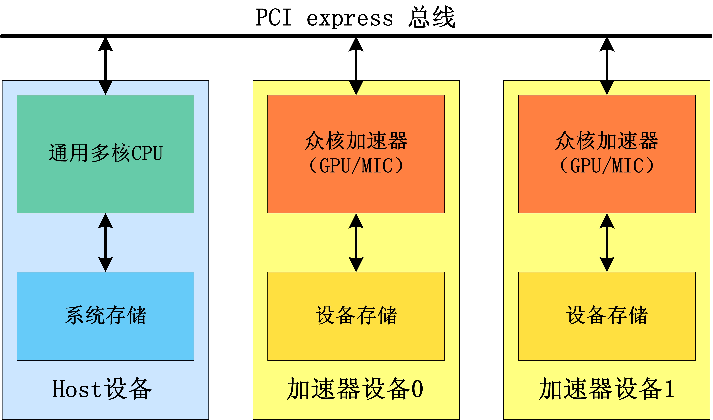
\includegraphics[width=0.7\linewidth]{figs/hybrid_sys}
	\caption{典型异构系统示意图}
	\label{fig:hybrid_sys}
        \end{figure}
       
       对于GPU加速器来说,应用的计算任务主要通过CUDA C来描述,这是一种并行执行模式,通过CUDA C描述的计算kernel代表了GPU中所有线程执行的行为,在CUDA C中,每个线程都有一个线程号,各个线程根据自己的线程号来访问不同的数据,CUDA提供线程编组的方式方便算法的设计。
       
       而与GPU不同的是,MIC加速器中内置了标量的x86核,第0号小核主要是运行一个微操作系统,因此MIC除了上述描述的主-从模式,还有两种执行模式:一种是MIC主导计算,MIC启动任务的执行,将部分适合标量处理器的任务交给主机CPU执行;另一种是CPU和MIC属于对等模式,将MIC看作一个独立的处理器,通过MPI启动多个进程分别在CPU和MIC上执行。
       
 \subsection{应用对高性能计算的迫切需求}
 科学计算等应用领域对计算能力的需求是推动并行计算机发展的动力\upcite{zhang2006parallel}。一系列重大挑战性的问题,如天气预报、核爆炸模拟、地震预测、生物医学等,每秒需要千万亿次浮点计算,需要处理的数据规模达到TB量级。传统的多核CPU系统无法满足这样的需求,只能通过大规模的并行计算得到解决。
 
 虽然当前的超级计算机系统的性能已经达到千万亿次(Peta-flops)浮点计算能力的时代,但很多应用,比如高能核物理、生命科学等对计算的需求达到百亿亿次级(Exascale)浮点计算,简称E级计算\upcite{E2014}。美国计算机科学中心选取了几个面向百亿亿级的程序\upcite{OLCF2011},如S3D、DENOVO、LAMMPS等,这些程序在不同的尺度下进行高分辨的数值模拟。由于这些应用对计算和模拟的时间空间分辨率、规模以及实时性的要求,使得它们对计算能力的需求永无止境。
 
 本课题选取两种应用实例在异构平台上进行研究,一个是心脏组织的模拟,该应用对计算的需求巨大,另一个是人工智能领域应用比较广的卷积神经网络计算,卷积神经网络的大规模训练具有对大规模并行计算的需求,本课题重点是在GPU异构平台下研究卷积神经网络前向计算过程。
 
 \textbf{1.  心脏组织模拟。}
 
并行计算在计算心脏学运用很广。计算心脏学对计算能力的需求在不停的增长,因为计算心脏学专家想采用高级的数学模型来模拟心脏并且在时间和空间上都使用更高的分辨率。由于异构超级计算机的超强计算能力,它们越来越受到欢迎。

计算心脏学中一个很重要的研究课题就是发生在心脏组织和器官级的心率失常。但由于有限的计算能力,大部分之前的研究只是集中在心脏细胞内电压行为以及钙离子处理的模型上,钙离子处理过程是通过对亚细胞中随机钙离子处理\upcite{gaur2011multiscale,nivala2012computational,restrepo2008calsequestrin,williams2011dynamics}离散化实现的。这些钙离子处理和电压行为的模型对于研究心率失常的起因和原理的研究非常有益。心率失常主要表现形式有后除级\upcite{GPUcell}和早后除级\upcite{nivala2012calcium,nivala2015t}。

但是将细胞级的研究推广到对组织或者器官级的心率失常是不够的,从模型到计算量都存在重大的挑战。人体的心脏大概有2 $\times$ $10^9$个细胞\upcite{adler1974cell},每个心脏细胞内又有$10^6$个RyRs(ryanodine receptors),这些RyR分布在大概$10^4$个钙离子释放单元中,每个dyad有15个L-type的通道,这些通道对电压和本地钙离子浓度做出反应\upcite{cheng1993calcium}。两个8核的Sandy Bridge CPU需要1秒钟去模拟3000个心脏细胞1个时间步。而由于一个现实的组织模拟涉及到$10^7$ $\sim$ $10^8$个细胞$10^4$ $\sim$ $10^5$个时间步,所以心脏模拟对超级计算的需求是很显然的。图\ref{fig:cardiac_level}为心脏模拟的自下而上的四个层次,分别从微观到宏观,对计算的需求逐渐增加。
\begin{figure}[ht!]
\centering
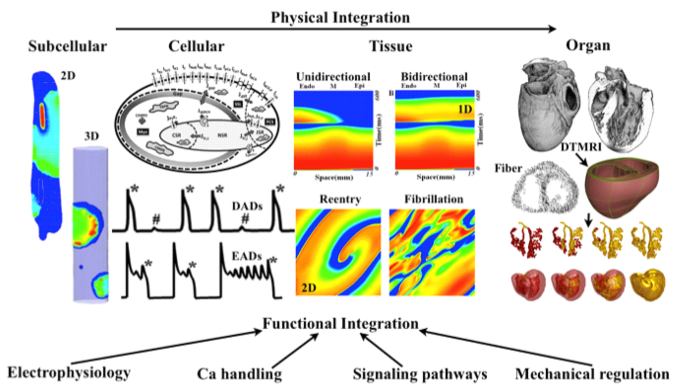
\includegraphics[width=0.9\linewidth]{figs/cardiac_level}
%\includegraphics[width=\linewidth]{figures/weak.PNG}
\caption{心电模拟自下而上的四个层次(从左到右是从微观到宏观)}
\label{fig:cardiac_level}
\end{figure}

 \textbf{2.  卷积神经网络应用与加速。}
 
对于卷积神经网络应用来说,用户希望能够尽快得到计算结果。而现有的神经网络却越来越复杂,如何在现有的硬件上实现一个低延迟的卷积神经网络变得尤为重要。卷积神经网络中的计算主要集中在卷积层,传统的卷积计算方法计算量大,特别是对于3D卷积计算来说,计算量和存储都会使现有的硬件资源无法满足。

为了降低卷积神经网络前向计算过程的延迟,采用异构GPU加速器进行加速,更重要的是改进算法,从卷积的算法实现上降低总的计算量,这对于加速卷积神经网络的计算过程具有重要的作用。本课题主要是针对3D卷积计算提出了新的3D卷积实现算法,该算法能够从理论上大幅度降低浮点计算量,并将新的3D卷积算法高效地映射到异构GPU体系结构中。

加速卷积神经网络前向计算过程还有一种方法就是采用多GPU设备并行的加速方案。而目前针对神经网络的多GPU加速方案主要采用的是数据并行方法,该方法可以有效提高神经网络处理的吞吐率,但无法降低神经网络的延迟。多GPU环境下,采用模型并行会带来通信问题,即在每层卷积层计算结束后,需要进行通信,通信开销与设备的数目成正比。因此设计一个高效的通信模式对性能影响也至关重要。

 
 \subsection{异构并行计算面临的挑战}
并行计算需要研究的内容包括并行体系结构、编译、算法、并行编程等\upcite{zhang2006parallel}。文献\upcite{Burkhard2010Some}中指出E级系统面临的五大挑战:访存、通信、可靠性、能耗、应用。通信、可靠性以及能耗会随着计算系统规模的增大而增大。异构系统可以称为E级系统的一种解决方案,因为异构系统中加速器的计算能力强,而功耗相对较低,由异构节点构成的E级系统规模可以变得更小,因此可以缓解通信、可靠性以及能耗的问题。异构体系结构带来的问题就是编程变得更加复杂,不更改代码,现在很难只通过更改硬件结构就能提升软件的性能,随着异构体系结构的出现,异构编程变得尤为复杂和重要\upcite{Sutter_the}。
 
异构系统为各种应用需求提供了很好的硬件基础。如何快速开发大规模并行程序,设计高效的并行优化方法,充分发挥异构系统的计算能力,成为当前并行计算研究的重大挑战。本课题根据真实的应用开发实践,总结了基于GPU/MIC异构系统的大规模并行程序设计面临的问题:
 
 \textbf{1. 异构计算资源利用不足。}
 
异构系统一般是由通用CPU+众核加速器构成的,CPU主要负责控制,CPU将应用中计算密集的部分加载到加速器中执行。而在很多超级计算系统或者服务器中,各个计算节点中的多核CPU功能一般都很强大,这是为了使系统更加通用。比如天河1A中的每个计算节点中安装了一个NVIDIA Tesla M2050 GPU和2个6核的Intel Xeon X5670 CPU(共12个CPU核)。天河1A中每个节点的CPU总性能与GPU性能的1/3相当。因此,如果只使用GPU进行计算,就会造成CPU计算资源的浪费。目前在某些应用领域,已有研究者研究基于GPU的异构系统中关于CPU和GPU协同计算的问题,如杨的Linpack实现\upcite{yang2010adaptive},卢的天气预报计算应用\upcite{lu2012cpu/gpu}。不过现在还没有一种统一的编程框架可以解决异构计算资源利用不足的问题,需要根据应用做专门的实现,本课题研究的心脏组织模拟还没有一个基于大规模异构平台的实现并且能充分利用CPU和加速器的计算资源。
 
  \textbf{2.  缺乏大规模异构系统上的性能量化研究。}
  
尽管异构系统应用开始变得广泛,但在TOP500榜单中占大部分比例的还是基于CPU的大规模同构系统,这是因为基于CPU的软件兼容性好,扩展到大规模同构系统时,性能好预测,而对于异构平台的软件,很难评估软件扩展到更大规模的异构系统中的性能,正是性能的不可预测性,阻碍了异构系统的推广和发展。对于心脏组织模拟的应用来说,之前的研究都是基于CPU的大规模系统,少量基于小规模的GPU异构系统研究,缺少在成百上千个异构节点上的研究实现,因此也无法对心脏组织模拟的真实性能进行预测。
 
   \textbf{3.  软件滞后硬件,某些应用还缺乏在新型异构系统上的实现。}
 应用领域的需求和新型加速器体系结构的发展相互促进,由于异构体系结构的独特特点,需要专门的编程模型,需要对应用重新并行开发。很多应用由于规模大,因此需要开发的周期长、成本高、难度大,如核物理软件CCSD由10名工程师开发了3年,气候软件由40人开发了20多年\upcite{E2014}。因此,平台移植所需的巨大工作量导致软件的开发滞后硬件。 而对于GPU平台来说,GPU呈现的复杂体系结构给编程带来了挑战。GPU中大量的并行计算单元支持很多硬件线程同时执行,Nvidia公司针对GPU专门开发了CUDA编程模型,根据CUDA编程模型,程序员可以描述每个线程的行为,以及控制CPU和GPU间的通信等功能,这些都为GPU编程带来了一定困难。此外,GPU提供丰富的存储层次满足计算对带宽的需求,如何通过编程来发挥各个存储层次的存储效率也是值得研究的问题。
 
 本课题关注的其中一种加速器类型就是Intel的第一代Xeon Phi众核加速器。Xeon Phi的双精度峰值性能是通过16*核数*频率计算的。比如1.053GHz 60个核的5110P协处理器具有的峰值性能可达16$\times$ 60 $\times$ 1.053=1011GFLOPS,这里的系数16是因为Xeon Phi的寄存器可达512位即8个双精度,并且每个核支持2个硬件线程。需要指出的是这里的峰值性能意味着使用了所有的硬件资源。
 
Xeon Phi能提供的巨大峰值性能给高效编程带来巨大的挑战。除了高效使用大量的硬件线程,程序员还需要关注如何发挥每个线程SIMD的能力。前者可以通过使用OpenMP编程来达到,SIMD向量化可以通过编译器的自动向量化或者使用AVX-512手动向量化来取得理想的8倍双精度浮点性能提升。

异构系统中另外一个不容忽视的因素是多核CPU的计算性能。目前,单个多核CPU的核数都是比较少的,通常在8到18之间,然而,每个CPU核都是高频的并且可以乱序执行,因此,CPU核比Xeon Phi的核的能力更强也更灵活。对于SIMD向量化不是很容易实现或者性能的瓶颈是存储带宽的非直接计算,一个典型的八核Sandy Bridge CPU可以取得与众核相当的性能。所以对于CPU+Xeon Phi的异构系统,同时发挥CPU和Xeon Phi的性能将变得很重要。异构计算除了给编程带来挑战,还涉及其它的任务,比如使用针对CPU核的256位的AVX指令集,对CPU和Xeon Phi间的通信进行优化以及两种不同硬件上负载均衡。
 
  \textbf{4.  缺乏基于新型节点内多MIC异构系统的混合计算编程框架。}
   
基于单个Xeon Phi加速器的编程和性能优化目前已经有很多研究,为了获得更强的性能,单节点内集成多个Xeon Phi加速器的异构系统成为一种解决方案,比如天河2号超级计算系统的每个节点内集成了3个Xeon Phi加速器和2个通用多核CPU。这样复杂的体系结构给编程带来了巨大挑战,主要有两个问题需要解决,一是多核CPU与Xeon Phis间的协同计算问题,二是CPU和Xeon Phi以及Xeon Phi间的数据传输问题。
 
本课题研究的心脏模拟应用任务比较规则,便于CPU与Xeon Phi间的任务划分,计算过程中涉及到通信等等,这些特点对于研究天河2号超级计算系统具有非常重要的意义。有利于在天河2号系统上开发一套混合编程框架,这对天河2号系统上其它应用的开发具有很好的指导意义。
 
 综上所述,基于GPU/MIC等新型加速器的高性能计算系统在对大规模应用的并行开发中具有很大的优势,这很好地促进了异构系统以及科学计算等应用的发展,同时也给研究人员带来了很多研究问题。这些问题直接影响到异构系统性能的发挥。本课题选取GPU和Xeon Phi这两种重要的加速器异构系统,通过两个应用实例研究基于异构系统的并行设计与实现技术,以及性能优化方法,为设计开发其它的异构混合计算应用积累经验并提供参考。


\section{研究意义}
本课题以心脏组织模拟这个科学计算为背景,采用多种并行优化手段将心脏组织模拟高效地 映射到超级计算机上比如天河 2 号。对于研究生物信息学领域的专家来说,验证他们 提出的心脏模型是否可靠,同时很多研究可以不用在具体的人身上做实验和观察,可以直 接通过改变参数做各种实验,这将极大地加速这方面的研究,所以,这对于心脏疾病的研 究具有重要的意义。

将真实的科学计算映射到天河 2 号异构计算平台,需要面临众多高性能计算的难题。 首先是需要提高单节点的性能,天河 2 号单节点内包括多核的 host CPU 以及 3 个 MIC 加速 卡,本课题采用 SIMD 向量化、OpenMP 以及 COI/SCIF 编程技术可以很好地解决天河 2 号 单节点各个计算单元的协同计算,以及很好地充分利用了各级并行。而在节点间采用 MPI 并行技术并且对 MPI 通信采取一定的优化措施,保证大规模异构节点的扩展性。所以本研 究的各项技术可以解决在天河 2 号上面向特定应用的编程问题,将使得天河 2 号在解决真实的科学计算问题上再向前迈一步。

基于GPU异构平台,采用新的卷积算法以及实现多GPU下的模型并行方法,能够有效加速卷积神经网络前向计算过程。同时这可以很好地提取卷积神经网络计算特征,并发现现有GPU体系结构在神经网络计算领域中存在的优势和不足,这对研究新型或者专用加速器具有重要的指导意义。

\section{研究现状}

\subsection{异构系统}
基于加速器的异构系统是指使用不同功能或性能的计算设备,通过一定结构互联而构 成的计算机系统,其中一种计算设备的计算能力强于传统的通用处理器,被称为加速器, 用于实现对应用程序需要密集计算部分的计算加速。典型的加速器包括数字信号处理器 (DSP)、面向通用计算的图像处理器(GPU)、众核协处理器(MIC)以及硬件加速器(FPGA) 等。

异构体系结构应用非常广泛,从各种嵌入式平台到高性能超级计算机,都采用了异构体系结构。QUALCOMM公司开发的Snapdragon 810嵌入式处理器\upcite{qualcomm}的峰值性能达到388Gflops,已经应用到手机和平板等各种嵌入式设备上。ARM 公司开发的 Mali-T760 \upcite{mali}嵌入式处理器峰值性能326GFlops。Imagination公司的PowerVR GT7900\upcite{powerVR}处理器峰值性能达552GFlops。NVIDIA 推出的 Jetson TX1 开发板\upcite{jetson}性能已经能达到 1TFlops。而在高性能计算领域,异构体系结构更是不可或缺。当时的天河-1号\upcite{tianhe1}超级计算机采用的是CPU+GPU的异构体系结构,而天河-2号\upcite{tianhe2}采用的是CPU+MIC的结构。采用异构系统的超级计算机还有Titan\upcite{titan}、Piz Daint\upcite{piz}以及Stampede\upcite{stampede}等。

\subsection{ 大规模异构系统编程模型}
大规模异构系统涉及到计算节点间的并行,节点内多个加速器与主机CPU间的并行,以及加速设备内部的并行。丰富的并行层次为编程模型提供了挑战,本节主要介绍基于GPU/MIC加速器的大规模异构系统的并行编程模型。节点间一般采用基于消息传递的MPI并行编程模型,对于基于MIC加速器的节点内部,CPU和MIC加速器间可以采用多种执行模式,比如offload模式,对等模式,native模式等,而MIC加速器上可以采用基于共享存储的OpenMP编程。对于基于GPU加速器的节点,可以采用CUDA并行编程模型,GPU上通过CUDA C语言对任务进行描述。
\subsubsection{消息传递编程模型}
消息传递编程模型主要是针对分布式存储系统中的一种并行编程模型,在分布式系统上创建进程,分布式系统间的消息传递通过进程间通信实现。这种消息传递模型通过进程执行相同或不同的代码实现并行(SPMD或MPMD),而进程间同步是通过栅栏同步完成的。消息传递机制的编程模型需要程序员显式控制数据传输,显式描述各个进程的执行任务,并且显式控制进程间的同步。这种编程方式虽然增加了程序员的负担,但具有很好的可移植性和可扩展性。消息传递编程系统主要包括MPI\upcite{mpistd}以及PVM\upcite{pvm}等,下面主要介绍MPI编程模型。

MPI是在串行程序的基础上扩展的,各种消息传递的接口构成了MPI并行编程环境。一个具体的MPI编程环境包括消息传递的接口函数以及学术界和工业界对这些函数的具体实现,如MPICH\upcite{MPICH}、LAM/MPI\upcite{LAMMPI}、MVAPICH\upcite{MVAPICH}、OpenMPI\upcite{OpenMPI}等。MPI具有良好的可移植性、可扩展性、可编程行、完备的异步通信功能等优点,使其成为最流行的并行编程语言。

\subsubsection{共享存储编程模型}
共享存储编程模型是基于共享存储并行机器模型上的细粒度线程级并行,它通过共享变量的读/写操作隐式实现并行线程间的数据通信。程序员通过对串行程序中计算量大的$for$循环部分使用编译指导语句,实现计算任务在线程间的隐式分配。对于线程间的异步执行,需显式执行多线程间的同步以确保程序的正确性。共享存储编程模型适合细粒度的并行开发,实现简单,只需要通过编译指导语句即可轻松实现并行程序。目前基于共享存储的编程模型中,流行的主要是OpenMP\upcite{dagum1998openmp}和Pthreads,OpenMP广泛用于高性能计算领域中的节点内部的并行。

OpenMP定义了一系列的编译指导命令,编译指导命令提供了对并行区域、变量的共享和私有、任务分配策略等支持,程序员只需要将这些编译指导命令应用到需要并行化的串行代码中,就能方便实现串行代码的并行化。OpenMP程序执行的原理是主程序首先串行执行到某个需要并行实现的地方,然后通过$fork-join$机制先创建多个并行程序执行需要并行执行的任务,并行执行的任务完成后,通过$join$合并成一个线程继续往前执行。对于大规模计算系统的节点是共享存储的多核节点,可以在节点上采用OpenMP进行并行实现。

基于共享存储的OpenMP编程模型可移植性不如MPI并行编程模型,但OpenMP更容易实现计算的并行化,并行编程的难度小,因此,同样也应用非常广泛。

\subsubsection{计算统一设备架构编程模型}
NVIDIA公司于2007年推出的CUDA(Compute Unified Device Architecture,计算统一设备架构)是专门针对NVIDIA GPU的编程模型\upcite{luebke2008cuda}。CUDA编程模型中,CPU为主机,GPU为协处理器,它们之间采用主从的执行模式,一个CUDA程序分成两部分,一部分是在CPU端执行的串行代码,另一部分是在GPU上执行的并行代码(称为kernel)。在CPU端执行的串行代码主要负责数据准备、设备初始化以及主机和设备间的数据传输。GPU上执行的kernel组织成线程网格(Grid),每个Grid又可划分成线程块(Block),每个Block又包含很多并发的线程(thread),Block映射到SM上执行,Block里的线程映射到CUDA核心中执行。CUDA采用SIMT的方式执行,多个Block可映射到同一个SM中,GPU通过专门的硬件动态调度Block到SM上执行。

CUDA编程模型为程序员暴露了很多硬件细节,因此,如果想要取得很好的性能,需要对硬件非常了解,针对硬件做相应的优化,一般主要通过三个方面提高CUDA程序的性能:一是应用支持足够多的并发线程隐藏延迟;二是合理利用GPU的存储层次;三是提高硬件的利用率。采用CUDA在GPU上对现有应用进行加速,能够取得很好的加速效果。

\subsubsection{通用异构并行编程模型}
OpenCL(Open Computing Language,开放计算语言)是一种通用的异构并行编程标准,是一种平台无关的编程模型\upcite{stone2010opencl}。目前支持OpenCL标准的硬件平台有CPU、GPU、DSP、Cell以及MIC等计算设备,由此可知,OpenCL程序具有很好的可移植性。

OpenCL程序与CUDA相似,也包括在主机上执行的控制代码和设备端执行的核心代码。主机端执行的代码也是负责初始化启动设备,准备数据和传输数据到计算设备中,计算设备端的代码负责对输入数据的并行处理,处理完任务后,将计算结果传输给主机端。在OpenCL编程模型中,计算设备被抽象成若干个并行计算单元,每个计算单元又由多个处理单元组成。计算设备中执行的代码通过核心(kernel)进行描述,kernel是通过线程来执行,每个线程也称为工作项(work item),多个工作项构成一个工作组(work group),工作组映射到计算单元中执行,工作项映射到处理单元中执行。

需要指出的是,虽然OpenCL程序具有很好的功能移植性,但性能移植性很差\upcite{wen2015improving},即针对某种设备优化好的OpenCL程序,移植到另一种设备上执行时,性能可能很差,这是因为不同设备体系结构相差很大,这就要求OpenCL程序需要针对专门的硬件设备做相应的程序优化,这同样对程序员要求比较高。文献\upcite{karimi2010a}对 CUDA 和 OpenCL 两种编程模型在GPU上的性能做了对比。

\subsubsection{MIC编程模型}
面向Intel MIC加速器平台\upcite{more2013intel},Intel提出了基于OpenMP语言进行编译制导扩展的MIC offload编程模型\upcite{Newburn2013}。MIC offload程序包括主机端的串行代码和加速设备上执行的并行代码组成,采用主从执行方式,通过offload编译制导进行标记。主机端代码完成MIC设备的启动以及数据的传输,被编译制导语句标记的那部分代码则在MIC设备端执行,在MIC端执行的代码可以继续使用OpenMP并行,根据MIC处理器中计算核心的数量创建足够多的线程来执行。

由于MIC核心中运算单元支持512位的SIMD向量化并行,因此,为了充分发挥硬件资源的利用率,需要使用向量化单元,有两种方法,一是通过编译器直接自动完成向量化,二是通过程序员使用向量化的汇编指令手动实现向量化。对于规则的计算,自动向量化的效果与手动向量化的效果一样,但对于一些不规则的计算,编译器无法完成自动向量化,此时需要通过手动向量化的方法完成向量化。

除了offfload模式外,还有对等模式以及本地执行模式。对等模式是将MIC处理器和CPU主机看成对等的计算节点,这使得原有大量的MPI+OpenMP应用程序可以不用修改直接在MIC处理器上直接运行。然而,鉴于MIC体系结构与CPU多核处理器的不同,为了使在MIC处理器上获得很高的性能,需要针对MIC处理器的特殊体系结构做相应的优化,如充分利用MIC的存储层次,充分发挥硬件多线程和向量单元的计算能力。

虽然应用开发人员都希望找到一种统一的编程模型,可以有效应对所有的硬件体系结构并且都能取得很好的性能,但这几乎不可能,因为不同处理器的硬件结构千差万别,针对不同的处理器做相应的优化是不可避免的。

\subsubsection{混合编程模型}
综上所述,不同的异构平台需要不同的并行编程模型,对于大规模异构系统,需要采用多种编程模型的混合模型,比如MPI+OpenMP,MPI+CUDA,MPI+OpenCL,MPI+OpenMP+CUDA,MPI+OpenMP+向量化等。混合编程模型包括多个层次,如图\ref{fig:hybrid_prog}所示,具体过程如下:1. 最上层在每个节点上运行一个MPI进程,任务通过MPI编程进行任务的一个粗粒度划分;2. 在节点内部可以通过OpenMP创建多线程实现多核并行;3. 针对节点内的协处理器,再采用某种专用编程模型(比如CUDA/OpenCL/MIC offload)进行并行编程。
\begin{figure}[ht!]
\centering
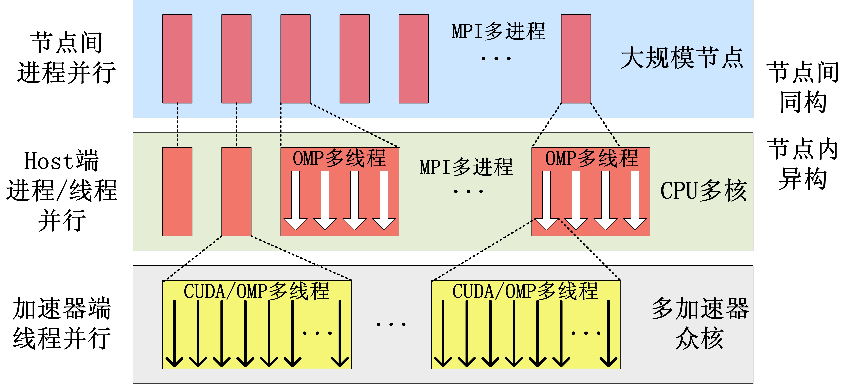
\includegraphics[width=0.8\linewidth]{figs/hybrid_prog}
\caption{大规模异构系统混合编程模型层次化视图(MPI+OpenMP+CUDA)}
\label{fig:hybrid_prog}
\end{figure}

\subsection{针对异构平台的并行优化技术研究}

%对异构系统的开发需要采用异构编程模型来实现。目前针对 NVIDIA GPU 主要采用 CUDA\upcite{luebke2008cuda}编程,也可以采用 OpenCL\upcite{stone2010opencl}编程。文献\upcite{karimi2010a}对 CUDA 和 OpenCL 两种编程模型在GPU上的性能做了对比。由于 OpenCL 是面向各种平台的框架,因此OpenCL的性能移植性\upcite{wen2015improving}并不是很好,针对不同的平台需要做专门的优化。针对 FPGA 异构平台的开发,目前已经开始支持OpenCL编程,这意味着FPGA开发的门槛将降低,但从目前看OpenCL在FPGA上的性能并不是很好。但只要随着FPGA对OpenCL的支持更加的完善,FPGA将成为一股新的热潮。Intel的众核协处理器 MIC\upcite{more2013intel}的编程模式可以有多种,比如有Native模式,这种方法可以直接将通用的C程序直接移植都 MIC 上。还支持 offload 模式\upcite{Newburn2013},Offload 模式有两种,一种是采用类似OpenMP\upcite{dagum1998openmp}的方法,在程序中添加一些编译指导语句,将核心计算部分加载到 MIC 中执行,另一种是采用 COI/SCIF\upcite{potluri2013mvapich-prism}编程,这是Intel提供的控制MIC的底层接口,编程将更加复杂,但效率会更高。

各种异构平台在不同应用中都发挥着重要作用。CPU+GPU的异构平台在QR矩阵分解\upcite{agullo2011qr}中取得了很好的效果,充分利用了CPU和GPU两种硬件资源。基于CPU+GPU的异构平台,Jun Chai\upcite{chai2013resource-efficient}充分利用计算资源解决了贝叶斯推断问题,在生物信息比对中,Bo Chen等人\upcite{chen2010a}将Smith-Waterman算法在GPU异构平台上进行了并行化实现,而Haidong Lan等人\upcite{lan2016parallel}在Xeon Phi的集群系统中实现了生物信息比对中的算法。Siddharth\upcite{choudhary2010practical}在异构GPU上实现了实时的3D重构。Joshua Peraza等人\upcite{peraza2013understanding}在Intel Xeon Phi上对stencil计算的性能进行了评估,而Jian Tao等人\upcite{tao2012using}采用GPU对stencil计算进行加速用于解决大规模的科学应用。异构平台在其它应用领域\upcite{chen2012accelerating, lu2015mrphi, conti2012gpu, junior2012a}也发挥着重要作用。

涌现了大量的针对异构计算的优化技术的研究。异构计算中需要解决多个重要问题,诸如异构平台中的CPU和加速器间的任务调度问题,文献\upcite{acosta2013dynamic}采用了一种动态的负载均衡策略,Ana Balevic等人针对异构平台中的数据流执行提出了流缓冲机制\upcite{streambuffer},Michela等人解决了异构平台下分布式存储中的数据调度问题\upcite{becchi2010data-aware},Alecio等人则提出了一种有效的动态调度运行时以及可调系统\upcite{binotto2011an},针对Intel Xeon Phi加速器的SIMD技术\upcite{tian2015effective}可以有效利用计算资源。

\subsection{心脏组织数值模拟的研究现状}
在组织级(tissue-level)来模拟心脏生物电行为对计算能力具有极大需求\upcite{niederer2011verification}。同时,复杂的心脏模型包含了上百个状态变量,因此需要强大和计算密集的解法来求解常微分方程(ODE)\upcite{hartman2002ordinary}。如果需要快速模拟,如几小时,来模拟整个心脏循环,就必须要使用非常大的并行计算机。文献\upcite{niederer2011simulating}中,通过在 16384个CPU 核上扩展并行而完成了对于人类心脏生物电生理的近实时的单域模拟(1 分钟之内)。随着使用能发挥大量并行的计算能力的,相对新的通用 GPU 的发展趋势,许多计算科学的领域以已经开始采用这种硬件技术。计算心脏学也无例外地使用了GPU 计算。文献\upcite{rocha2011accelerating}中对于 2 维度心脏模拟,对心脏细胞膜的单域方程和 ODE 在GPU 上进行了求解,获得相对于 4 核 CPU 的 20 倍的加速。Bartocci 等人\upcite{bartocci2011toward}展示了使用单个 GPU,通过仔细的和面向模型的优化,包括真实和细节化的心脏细胞模型的 2 维 /3 维模拟能够以接近实时执行。之前的已有研究单域心脏模拟使用少量的 GPU。在文献\upcite{sato2009acceleration}中,使用 4 个 GPU 的心脏单域模拟 3 维代码展示了相比 32个 CPU 核的 1.6 倍加速。Vigmond 等人\upcite{vigmond2009near-real-time}展示了对于求解心脏单域模型的一套非线性的 ODE,相比 4 个 CPU 核,在 4 个 GPU 上能够加速 9–17 倍。在文献\upcite{nimmagadda2012cardiac}中,心脏双域模拟被移植到一个 4 GPU 的平台,对于基本的显式的数值方法进行了有效的面向体系结构的优化,并通过细粒度的并行策略,使得对于 3 维模拟相比单个 CPU 核获得巨大的改进(加速比 2460)。在文献\upcite{neic2012accelerating}中,通过使用当前主流的兔子心室模型,展示了心脏双域模拟运行在 6–20 个 GPU 上能够获得的性能好处和扩展性。对于并行化一个 2 维单域模型,最近的工作就是使用混合CPU-GPU的方法,展示了当运行于 8 节点的阵列时,相比只有 CPU 的实现(使用 64 个CPU 核),混合实现(使用 64 个 CPU 核以及 16 个 GPU)获得了近似 7 倍的加速\upcite{barros2012simulations}。

 纳米精度的亚细胞级钙动力数值模拟可以作为一个重要的工具,用于探索很多心脏疾病的生理原因。现有研究已经建立了很多计算模型,通过计算模拟来更好地理解钙信号以及钙波动产生的复杂动力学过程\upcite{izu2013ca2+}。然而,基本的挑战来自于其中包括极其不同的长度量级:t-细管和 SR 之间的裂缝范围在 10 nm以内\upcite{franziniarmstrong1999shape, hayashi2009three-dimensional},单个 RyR 的通道口是 1 nm大小\upcite{serysheva2005structure},而细胞规模从 10 到 100 µm 不等。当前建立的亚细胞钙波动生成模型为了研究整个细胞,而对钙动力学折中了部分细节\upcite{nivala2012computational},且只模拟到 0.2um 的网格精度。他们将一个 CRU 的动力学与单个的随机变量相结合,来代替对单独 RyR 的随机调整。即无论何时钙离子释放发生,他们都将其作为单点的来源。当前的模拟研究主要障碍之一就是巨大的计算需求。例如,为了在单个肌纤维节内求解纳米级规模的 CRUs,会占用一个体积为 10 × 10 × 2$µm^3$ 的 3 维空间,需要 2 × 1011 个体积单元, 每个单元的体积为 1 $nm^3$。体积单元的数量总是伴随这巨大数量的时间步需求。为了模拟一个肌纤维 1 ms,可能需要总的浮点操作数在$10^{19}$的量级\upcite{chai2015towards}。因此使得亚细胞钙动力学在纳米精度的模拟极具挑战性。已有的研究或者去掉细节,或者只模拟非常小的空间域,欠缺实际物理意义。而真实的研究最理想的是包括多个肌纤维节,并模拟超过数百毫秒。由此可见,在可预见的未来,在纳米精度下亚细胞级钙动力学模拟都将是一个极具挑战性的课题。

\subsection{卷积神经网络快速实现的相关研究}

随着卷积神经网络变得越来越复杂,计算量越来越大,异构平台成为卷积神经网络实现的有效平台。目前主流的异构平台主要是GPU、FPGA以及TPU,GPU平台主要优点是编程简单,加速效果明显,FPGA平台的峰值性能一般没有GPU高,但效率高,能耗低,在某些场景下具有优势,TPU是Google公司专为神经网络设计的加速器,在神经网络的计算过程中,可以达到很高的峰值性能。

在GPU异构平台上针对卷积神经网络进行加速的工作已经很多了。文献\upcite{krizhevsky2014one}对卷积神经网络在GPU异构平台上进行了并行化,文献\upcite{scherer2010accelerating}在GPU异构平台上对卷积神经网络的训练过程进行加速,最后取得了很好的加速效果,文献\upcite{strigl2010performance}将卷积神经网络中计算密集的部分分配到GPU中进行加速,在GPU中能够取得很好的性能和可扩展性。文献\upcite{paine2013gpu}在GPU平台中实现了异步随机梯度下降法对神经网络的训练过程进行加速。由于神经网络结构越来越复杂,对神经网络的训练也由单节点转向多节点,文献\upcite{coates2013deep}中的工作是基于GPU集群环境下进行训练的,能够扩展到16个节点中进行训练,而Awan等人提出设计的S-caffe框架\upcite{scaffe}将Caffe\upcite{jia2014caffe}扩展成了多节点版本,并对多节点环境下进行了通信方面的优化,最后在160个GPU上取得了很好的扩展性。

基于FPGA的神经网络加速的相关研究也逐渐变得流行起来。Chen Zhang等人\upcite{zhang2015optimizing}针对现有的FPGA加速器在实现神经网络中空间没有得到充分利用,并且计算吞吐率与带宽存在不能匹配的问题,他们根据roofline模型\upcite{williams2009roofline}提出了一个定量分析的方法论证了在最少使用FPGA资源的情况下完成计算任务。文献\upcite{sankaradas2009a}中的工作主要是将卷积神经网络中中的涉及到的计算都在FPGA中实现了,采用低精度的数据表示来增加有效存储带宽。Yuran Qiao等人\upcite{qiao2016fpga‐accelerated}在FPGA上高效地实现了一个矩阵乘模块,并将该模块用于解决卷积神经网络的卷积层计算,取得了很好的性能,文献\upcite{2017arXiv170103534A}采用OpenCL高级语言在FPGA上进行开发,实现对神经网络的加速。文献\upcite{li2016a, DataflowFPGA}中工作也是基于FPGA对卷积神经网络的加速。

还有加速卷积神经网络的方法是简化神经网络中的计算。Mathieu等人采用傅立叶变换的方法\upcite{mathieu2013fast}实现卷积计算,这种方法在卷积核大小比较大的时候优势明显,因为卷积核大小在一定范围内变化时,比如3~16,傅立叶方法所需的计算量不会随着卷积核大小变化而变化,而对于传统卷积方法来说,卷积核越大意味着卷积所需的计算量越大,因此,在卷积核比较大时,选择傅立叶方法在计算量方面有明显的优势,而傅立叶方法存在的问题就是所需的存储开销大,这成为限制傅立叶方法普遍使用的重要障碍。Lavin等人\upcite{lavin2016fast}将一个称为Winograd的算法应用在2D卷积计算中,并且在GPU平台上高效地实现了Winograd算法。Winograd算法是传统卷积计算方法与傅立叶方法的一种折中,即在保持存储开销不变的条件下降低计算量,最后的实验结果也表明,他们在GPU上的高效实现最后性能超过目前最快的cuDNN库。Winograd算法也非常适合在硬件加速平台上实现,Aydonat等人\upcite{aydonat2017opencl}就将Winograd算法在FPGA平台上采用高级语言进行了实现。另一种加速卷积网络计算的思路是将其中的浮点计算转化为代价更小的计算类型。比如将32位的浮点运算转化为16位浮点或者8位浮点运算,而这基本不会影响结果的精度。有些工作\upcite{courbariaux2015binaryconnect}、\upcite{courbariaux2016binarized}甚至将卷积计算的输入和模型参数转化为4位或者2位。而Rastegari等人\upcite{rastegari2016xnor}提出了一个XNOR网络,这个网络的输入和模型参数都是用1位来表示,而它们之间的计算则转化为异或计算,这些方法不但简化了计算而且还节省了存储开销,但存在精度下降的问题。

\section{主要研究内容和创新点}
异构平台在科学计算和人工智能领域逐渐发挥越来越重要的作用。本课题分别从科学计算和人工智能领域各选取一个典型应用即心脏组织模拟和卷积神经网络在异构平台上进行映射。无论是心脏组织模拟应用还是卷积神经网络应用,对计算需求都非常大,其中包含的计算也有各自的特点,根据计算特点,本课题选取了两种典型的异构平台进行实现,一种是基于Intel Xeon Phi加速器的异构平台,一种是基于GPU的异构平台。主要涉及的研究内容包括以下几方面:
\begin{compactitem}
\item[1.]心脏组织的3D模拟在大规模多核CPU系统上的映射。本课题提出了一个精细的3D心脏组织模拟模型,这个模型能够模拟人类心脏组织细胞内的电活动和钙离子处理过程。本课题最终是要将心脏组织的3D模拟映射到大规模异构系统中,具体的系统为天河2号系统,对于大规模异构集群系统来说,各节点的主机CPU的性能也不能忽略,因此本课题首先针对大规模集群的多核CPU系统进行优化。

\item[2.]心脏组织模拟的3D模拟在天河2号超级计算系统上的映射。针对Intel Phi加速器采用多种并行技术对心脏组织模拟中的核心计算进行并行优化,根据异构平台体系结构的特点实现了tissue level、cell level以及dyad level的三级并行。

\item[3.]3D卷积神经网络在异构GPU平台上的高性能实现。针对目前3D卷积网络中卷积计算量大的特点,推导出了一种能够有效降低计算量的3D卷积算法,即3D Winograd算法。本课题从理论上证明了该算法能有效降低浮点运算量,并在GPU异构平台上高效地并行实现,最后取得了比当前流行的深度学习库更好的性能。

\item[4.]面向卷积神经网络前向过程的低延迟实现。低延迟作为卷积神经网络前向过程的一个重要指标,为了降低计算时间,本课题在多GPU设备上对卷积神经网络采用模型并行。模型并行需要解决设备间的通信问题,因此,本课题还需要设计一个高效的通信模式,一方面降低通信时间,另一方面尽量隐藏通信时间。

\end{compactitem}

创新点有以下几点:
\begin{compactitem}
\item[1.]提出了心脏组织细胞的精细数学模型并且实现一个基于大规模多核CPU系统的心脏组织的3D模拟器。能够模拟一定规模的心脏组织的一些简单行为。

\item[2.]面向天河2号异构系统,实现了一个大规模心脏组织的3D模拟器。实现了心脏组织模拟的多级并行,很好地将个部分计算映射到异构集群系统中。

\item[3.]面向GPU异构计算平台,设计和实现了一个快速的3D卷积算法。本课题首次推导和实现了该快速算法的3D形式,并从理论上论证了该算法能够有效降低计算量。

\item[4.]面向多GPU设备,采用模型并行完成了卷积神经网络前向计算过程的低延迟实现。设计了一种环形的通信结构,使得通信开销不会随着GPU设备数目的增多而变得复杂,并且实现了通信与计算的重叠执行。

\end{compactitem}

\section{论文结构}
本论文共分为六章,具体结果介绍如下:

第一章为绪论,主要介绍本课题研究的背景和意义,并对本课题研究的两个典型应用\pozhehao 心脏组织模拟和卷积神经网络加速方面以及面向异构平台的并行优化技术方面的相关研究进行了介绍。

第二章首先介绍了心脏组织的数学模型、心脏细胞的数学模型以及对应的数值方法,然后介绍了心脏组织和细胞的数学模型在多核CPU系统上的并行映射实现。

第三章介绍将心脏组织和细胞的数学模型映射到天河2号系统中,主要介绍了映射过程中的具体并行技术。在实验部分介绍了心脏组织模拟在天河2号系统上单节点的性能以及多节点上的扩展性结果。

第四章介绍基于GPU异构平台下的3D卷积神经网络的快速算法实现。介绍了3D卷积神经网络的快速算法原理、该算法的复杂度分析以及面向GPU异构平台的并行实现。

第五章介绍了在多GPU环境下降低卷积神经网络前向计算过程延迟的方法以及一种通信开销不随GPU数目增多而增大的通信模式设计。此外,还介绍了通信与计算重叠技术的实现。





